% How the dataset is made: the diagram in the README (docs/dataset_pipeline.png).
% Rebuild: pdflatex dataset_pipeline.tex && pdftoppm -png -r 220 -singlefile dataset_pipeline.pdf dataset_pipeline
\documentclass[11pt,border=6pt]{standalone}
\usepackage[T1]{fontenc}
\usepackage[utf8]{inputenc}
\usepackage{lmodern}
\usepackage{amsmath}
\usepackage{xcolor}
\usepackage{tikz}
\usetikzlibrary{positioning,arrows.meta,calc,fit,backgrounds,shadows}
\begin{document}
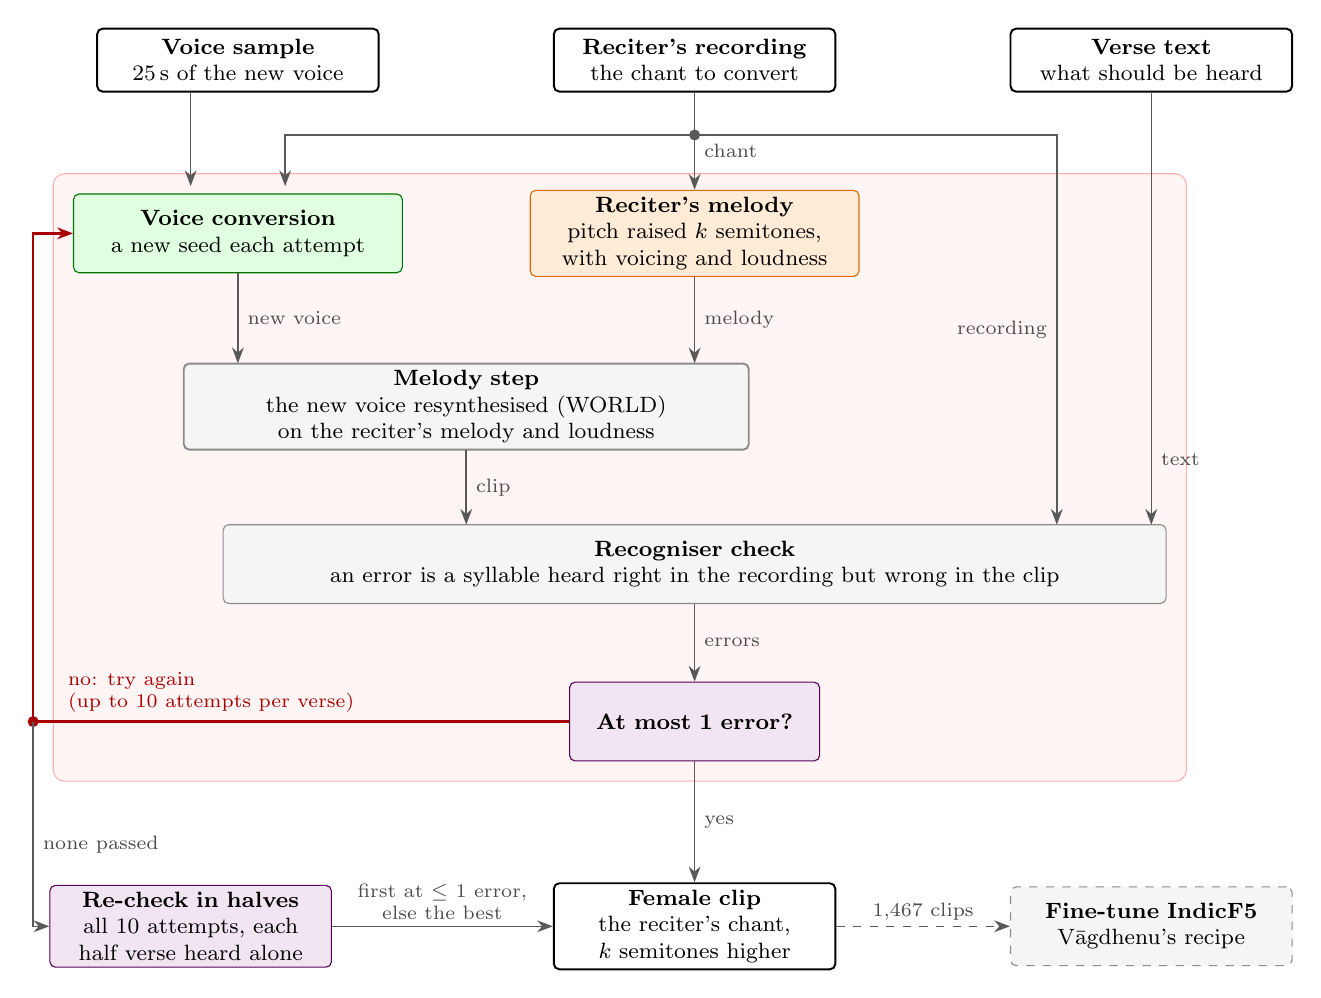
\begin{tikzpicture}[
  font=\footnotesize,
  x=1mm, y=1mm,
  >={Stealth[length=2mm]},
  box/.style={draw=black!45, fill=black!4, rounded corners=2pt, align=center, minimum height=10mm, text width=34mm, inner sep=2.5pt},
  input/.style={box, draw=black, fill=white, line width=0.7pt, minimum height=8mm},
  conv/.style={box, draw=green!45!black, fill=green!12},
  his/.style={box, draw=orange!85!black, fill=orange!16},
  keep/.style={box, draw=violet!70!black, fill=violet!10},
  flow/.style={->, draw=black!65, line width=0.55pt},
  loopflow/.style={->, draw=red!65!black, line width=0.9pt},
  lab/.style={font=\scriptsize, text=black!70, inner sep=1pt, align=left},
  side/.style={lab, right=0.8mm},
  loopbg/.style={fill=red!4, draw=red!30, rounded corners=4pt}]

% Inputs
\node[input] (voice) at (0,0)   {\textbf{Voice sample}\\25\,s of the new voice};
\node[input] (rec)   at (58,0)  {\textbf{Reciter's recording}\\the chant to convert};
\node[input] (text)  at (116,0) {\textbf{Verse text}\\what should be heard};

% One attempt: conversion, melody step, recogniser, decision
\node[conv, text width=40mm] (vc)     at (0,-22)  {\textbf{Voice conversion}\\a new seed each attempt};
\node[his, text width=40mm]  (world)  at (58,-22) {\textbf{Reciter's melody}\\pitch raised $k$ semitones,\\with voicing and loudness};
\node[box, line width=0.7pt, text width=70mm] (melody) at (29,-44)
  {\textbf{Melody step}\\the new voice resynthesised (WORLD) on the reciter's melody and loudness};
\node[box, text width=118mm] (asr) at (58,-64)
  {\textbf{Recogniser check}\\an error is a syllable heard right in the recording but wrong in the clip};
\node[keep, text width=30mm] (decide) at (58,-84) {\textbf{At most 1 error?}};

\begin{scope}[on background layer]
  \node[loopbg, fit=(vc)(melody)(asr)(decide), inner xsep=2.5mm, inner ysep=2.5mm] (loop) {};
\end{scope}

% Inputs into the attempt
\draw[flow] (voice.south -| -6,0) -- (-6,-16);
\draw[flow] (rec) -- node[side, pos=0.6]{chant} (world);
\draw[flow] (58,-9.5) -| (6,-16);
\draw[flow] (58,-9.5) -| node[lab, pos=0.75, left=0.8mm]{recording} (104,-59);
\fill[black!65] (58,-9.5) circle (0.7);
\draw[flow] (text.south) -- node[side, pos=0.85]{text} (116,-59);

\draw[flow] (vc.south) -- node[side]{new voice} (0,-38.5);
\draw[flow] (world.south) -- node[side]{melody} (58,-38.5);
\draw[flow] (29,-49.5) -- node[side]{clip} (29,-59);
\draw[flow] (asr.south) -- node[side]{errors} (decide.north);

% Retry: next seed
\draw[loopflow] (decide.west) -- (-26,-84) |- (vc.west);
\node[lab, anchor=south west, text=red!65!black] at (-22,-83.3) {no: try again\\(up to 10 attempts per verse)};

% Out of the attempts
\node[keep, text width=34mm] (halves) at (-6,-110) {\textbf{Re-check in halves}\\all 10 attempts, each half verse heard alone};
\node[input, minimum height=10mm] (clip) at (58,-110) {\textbf{Female clip}\\the reciter's chant, $k$ semitones higher};
\node[box, dashed] (model) at (116,-110) {\textbf{Fine-tune IndicF5}\\Vāgdhenu's recipe};

\draw[flow] (decide.south) -- node[side]{yes} (clip.north);
\fill[red!65!black] (-26,-84) circle (0.7);
\draw[flow] (-26,-84) |- node[lab, pos=0.3, right=0.8mm]{none passed} (halves.west);
\draw[flow] (halves) -- node[lab, above=1pt, align=center]{first at $\le$ 1 error,\\else the best} (clip);
\draw[flow, dashed] (clip) -- node[lab, above=1pt, align=center]{1,467 clips} (model);
\end{tikzpicture}
\end{document}
